	\begin{enumerate}[label=\alph*)]
		\item Queremos calcular el potencial electrostático y el campo eléctrico en el interior del semiconductor. Usamos la misma relación que en el ejercicio anterior:
		\begin{equation}
			\Ecal = \frac{1}{q} \derivadas{E_i}{x}
		\end{equation}
		Veamos que la energía varía como:
		\begin{equation}
			E_i(x) = \left\lbrace \begin{array}{ll}
				\frac{E_{i0}}{L/3-x_1} (x-x_1) \quad & \ \text{si} \ x<L/3 \\
				E_{i0} \quad & \ \text{si} \ L/3<x2L/3 \\
				E_{i0+\frac{E_{i0}}{L/3-x_1} (x-2L/3)} \quad & \ \text{si} \ 2L/3<x
			\end{array} \right.
		\end{equation}
		Recordamos que en $L/3$ tenemos que $E_v=-E_g/3$, y por tanto $E_c=2E_g/3$, tal que $E_{i0}=E_g/6+(3kT/4)\cdot \log(m_n^*/m_p^*)=0.179 \ \eV$, donde hemos redefinido $E_F=0$. Por lo que igual que antes tenemos que el campo eléctrico viene dado por regiones:
		\begin{equation}
			\Ecal(x) = \left\lbrace \begin{array}{ll}
				\frac{E_{i0}}{L/3-x_1} \quad & \ \text{si} \ x<L/3\\
				0 \quad & \ \text{si} \ L/3<x2L/3 \\
				\frac{E_{i0}}{L/3-x_1} \quad & \ \text{si} \ 2L/3<x
			\end{array} \right.
		\end{equation}
		y por tanto:

		\begin{equation}
			V(x) = \left\lbrace \begin{array}{ll}
				V_0 -\frac{E_{i0}}{L/3-x_1} (x-L/3) \quad & \ \text{si} \ x<L/3 \\
				V_0 \quad & \ \text{si} \ L/3<x2L/3 \\
				V_0 -\frac{E_{i0}}{L/3-x_1} (x-2L/3) \quad & \ \text{si} \ 2L/3<x
			\end{array} \right.
		\end{equation}
		Ahora solo tendríamos que hacer el esquema:
	
		\begin{center}
			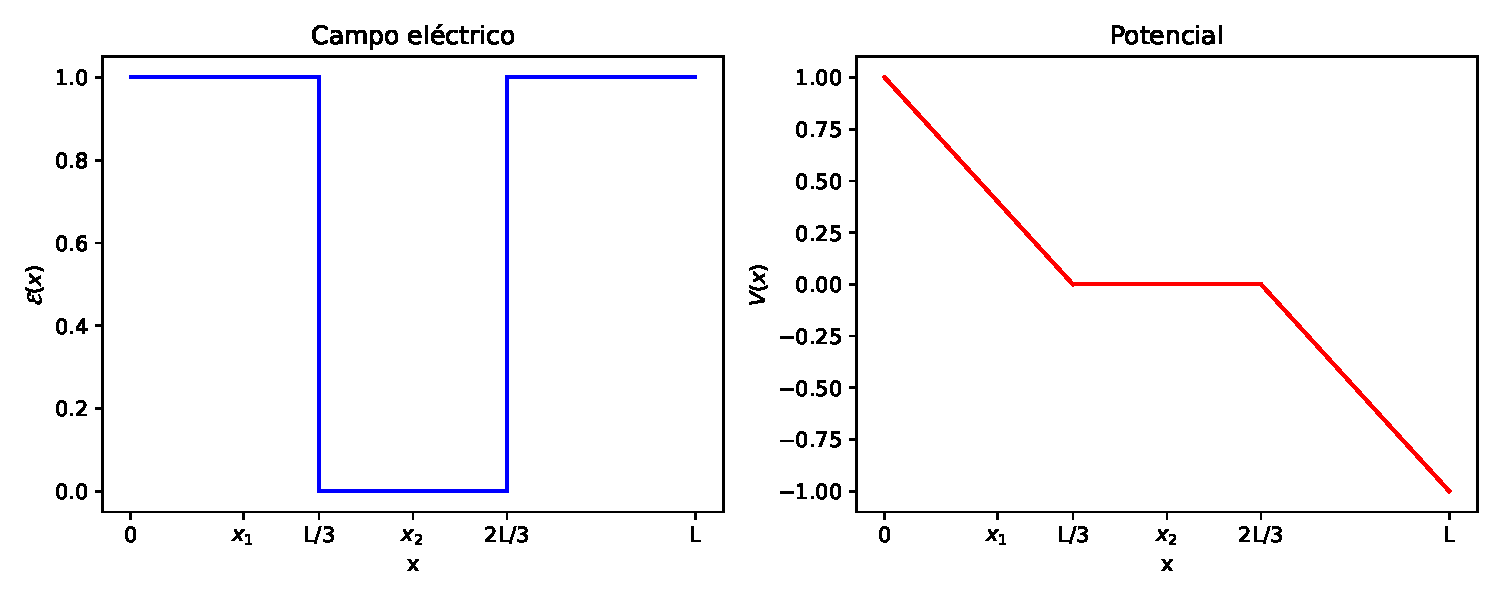
\includegraphics[width=\linewidth]{Cuerpo/Ch_02/02_Ejercicio_16.pdf}
		\end{center}
			
		Para determinar que está en equilibrio basta ver que $\Jn_T=0$ y que $T=\cte$, lo cual es cierto. Para ver que $\Jn=0$ debemos seguir el mismo procedimiento que antes.
		\item  Evidentemente es degenerado en $x=L$, ya que $E_F=E_v$. En $x_2$ tenemos que:
		\begin{equation}
			p = N_V e^{\frac{E_F-E_v}{kT}} = N_V e^{\frac{E_g}{3kT}} = n_i e^{\frac{E_F-E_i}{kT}}
		\end{equation}
		tal que en $x_2$ tenemos que $E_i=E_{i0}=0.179 \ \eV$. Los datos:

		\begin{equation}
			p = 1.22 \times 10^{13} \ \cm^{-3}
		\end{equation}
		\item Nos piden la densidad de corriente de electrones $J_n$ y la densidad de corriente de huecos en $x=x_1$. Es exactamente igual que en el anterior ejercicio:
		\begin{equation}
			\Jn|_{\text{{arrastre}}} = q \mu_n n \Encal = 0
		\end{equation}
		ya que en $x_1$ no hay corriente. La energía cinética del hueco $T$ viene dada por la diferencia entre $E_v=0$ (en $x=L$) y $-E_g/3$. Así pues:

		\begin{equation}
			T = - \frac{-E_g}{3}
		\end{equation}
		por suponer, ya que no tenemos ningún tipo de motivación para suponer que es así.

	\end{enumerate}
